\subsection{Directional lighting} \label{subsec:directional-lighting}
During the in-game daytime, the directional light is used to represent the light cast by the sun.
The light direction $l$ is the vector pointing toward the sun.
During the night the directional light is much dimmer but still present.
In this case, the light direction $l$ is pointing toward an imaginary light source ("the stars") which is rotating along with the sky.
\autoref{fig:directional-light} shows the terrain and other game objects illuminated by the directional light of orange color.
\begin{figure}[!htb]
    \centering
    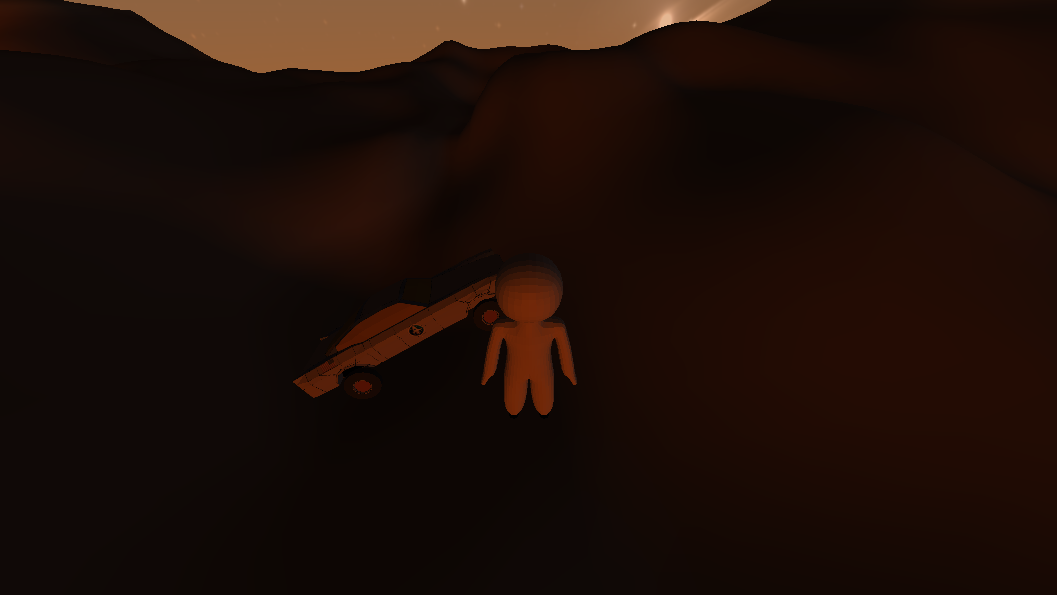
\includegraphics[width=0.8\textwidth]{chapters/theoretical_foundations/sections/lighting/resources/directional-light.png}
    \caption{Directional light}
    \label{fig:directional-light}
\end{figure}